\section{Planteamiento del desarrollo del proyecto}
El desarrollo de este proyecto se centra en la implementación de una red social simulada basada en grafos. Los nodos representan perfiles de usuario y los bordes, sus conexiones (seguidores y seguidos). Los algoritmos principales empleados incluyen:

\begin{itemize}
    \item Similitud de Jaccard: Implementado para calcular la semejanza entre los intereses o conexiones de diferentes usuarios.
\end{itemize}

El proyecto incorpora una estructura modular, separando tareas como el almacenamiento de datos en archivos, la simulación de conexiones entre usuarios y el cálculo dinámico de métricas para optimizar el rendimiento.

Para la implementación del índice de Jaccard, se utilizó una tabla hash para las listas de preferencias de cada usuario. Esto permite comparar eficientemente las preferencias de dos usuarios y calcular el índice de Jaccard.

A continuación, se presenta un ejemplo gráfico de la implementación de la similitud de Jaccard:


\begin{figure}[H]
    \centering
    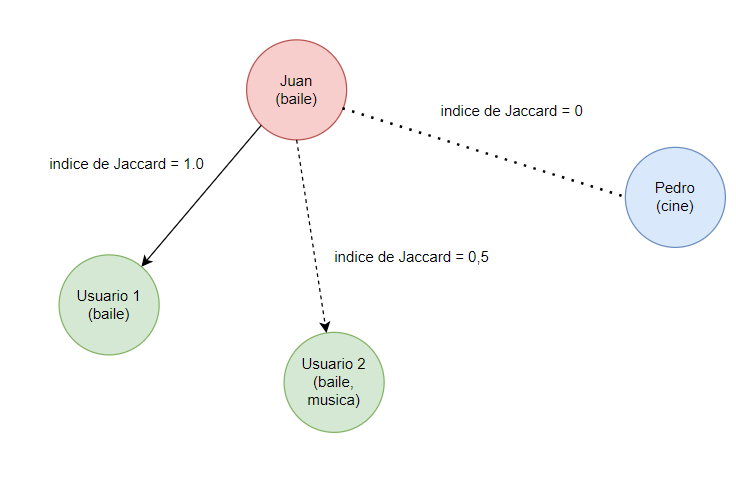
\includegraphics[width=0.5\textwidth]{src/figures/Jaccard.png}
    \caption{Ejemplo gráfico de la implementación de la similitud de Jaccard.}
    \label{fig:uniqueJaccard}
\end{figure}